\documentclass{article}
% Change "article" to "report" to get rid of page number on title page
\usepackage{amsmath,amsfonts,amsthm,amssymb}
\usepackage{setspace}
\usepackage{fancyhdr}
\usepackage{lastpage}
\usepackage{extramarks}
\usepackage{chngpage}
\usepackage{soul}
\usepackage[usenames,dvipsnames]{color}
\usepackage{graphicx,float,wrapfig}
\usepackage{ifthen}
\usepackage{listings}
\usepackage{courier}
\usepackage{upquote}

\definecolor{MyDarkGreen}{rgb}{0.0,0.4,0.0}
\newcommand{\ComplexUnit}{\ensuremath{\mathrm{i}}}

% For faster processing, load Matlab syntax for listings
\lstloadlanguages{Python}%
\lstset{language=Python,
        frame=single,
        basicstyle=\small\ttfamily,
        keywordstyle=[1]\color{Blue}\bf,
        keywordstyle=[2]\color{Purple},
        keywordstyle=[3]\color{Blue}\underbar,
        identifierstyle=,
        commentstyle=\usefont{T1}{pcr}{m}{sl}\color{MyDarkGreen}\small,
        stringstyle=\color{Purple},
        showstringspaces=false,
        tabsize=5,
        % Put standard Python functions not included in the default
        % language here
        morekeywords={},
        % Put Python function parameters here
        morekeywords=[2]{},
        % Put user defined functions here
        morekeywords=[3]{},
        morecomment=[l][\color{Blue}]{...},
        numbers=left,
        firstnumber=1,
        numberstyle=\tiny\color{Blue},
        stepnumber=5
        }

% In case you need to adjust margins:
\topmargin=-0.45in      %
\evensidemargin=0in     %
\oddsidemargin=0in      %
\textwidth=6.5in        %
\textheight=9.0in       %
\headsep=0.25in         %

%% % Homework Specific Information
%% \newcommand{\hmwkTitle}{One}
%% \newcommand{\hmwkSubTitle}{Two}
%% \newcommand{\hmwkDueDate}{Three}
%% \newcommand{\hmwkClass}{Four}
%% \newcommand{\hmwkClassTime}{Five}
%% \newcommand{\hmwkClassInstructor}{Six}
%% \newcommand{\hmwkAuthorName}{Seven}

%% % Setup the header and footer
\pagestyle{fancy}                                                       %
%% \lhead{\hmwkAuthorName}                                                 %
%% \chead{\hmwkClass\ (\hmwkClassInstructor\ \hmwkClassTime): \hmwkTitle}  %
%% \rhead{\firstxmark}                                                     %
\lfoot{\lastxmark}                                                      %
\cfoot{}                                                                %
\rfoot{Page\ \thepage\ of\ \protect\pageref{LastPage}}                  %
\renewcommand\headrulewidth{0.4pt}                                      %
\renewcommand\footrulewidth{0.4pt}                                      %

\title{Coherent population trapping with pulsed laser,\\the notes}
\author{Greg}
\date{version 0.1, \today}

\begin{document}
\begin{spacing}{1.1}
\maketitle
% Uncomment the \tableofcontents and \newpage lines to get a Contents page
% Uncomment the \setcounter line as well if you do NOT want subsections
%       listed in Contents
%% \setcounter{tocdepth}{1}
\tableofcontents
\newpage


\section{Introduction}
This note supposed to summarize the current status of the Bloch-equation calculation towards explaining the frequency-comb Coherent Population Trapping (CPT) experiment. It starts in the very beginning, because there is a lot to learn. For most of the calculations I adopt notation that is convenient for me. If I have to convert from the notation of e.g. a paper, I give the method of conversion too. 

A single element of the a density matrix is a complex number. For many calculations it is more convenient to use only real numbers, thus we separate the real an imaginary component.
\begin{equation}
\rho_{kl} = x_{kl} + y_{kl} \ComplexUnit
\end{equation}
The diagonal elements of the density matrix are called populations, while the off-diagonals are the coherences. Since the density matrix has is Hermitian, the populations are real numbers, while the coherences are generally complex.

The simplest Bloch equations are written in the following form, for the time derivative of the  populations, and the real / imaginary part of the coherences:
\begin{subequations}
\begin{align}
\dot x_{jj} &= \sum_{l=1}^N (2 M_{lj} y_{jl} + A_{jl} x_{ll}) - \gamma_j x_{jj} \\
\dot x_{jk} &= \sum_{l=1}^N (- M_{jl} y_{lk} + y_{jl} M_{lk}) - x_{jk} \left(\frac{\Gamma_j + \Gamma_k + \Gamma_{L,jk}}{2}\right) + y_{jk} \Delta_{jk} \\
\dot y_{jk} &= \sum_{l=1}^N (  M_{jl} x_{lk} - x_{jl} M_{lk}) - y_{jk} \left(\frac{\Gamma_j + \Gamma_k + \Gamma_{L,jk}}{2}\right) - x_{jk} \Delta_{jk}
\end{align}
\end{subequations}

A note about the $\Delta$ detunings: in general $\Delta_{jk} = \Delta_{jl} + \Delta_{lk}$ with $\Delta_{ij} = - \Delta_{ji}$ and blue detuning is positive.


\section{Repeating results from other papers}

\subsection{Basic three level system}
From my precious group, Matt McDonnel's thesis \cite{McDonnell2003}
Figures 4.3, 4.5, 4.6, 4.7. Correction, time is scaled as $1/\Gamma$, not as in the thesis claimed as $2\pi/\Gamma$.

\begin{figure}
\begin{center}
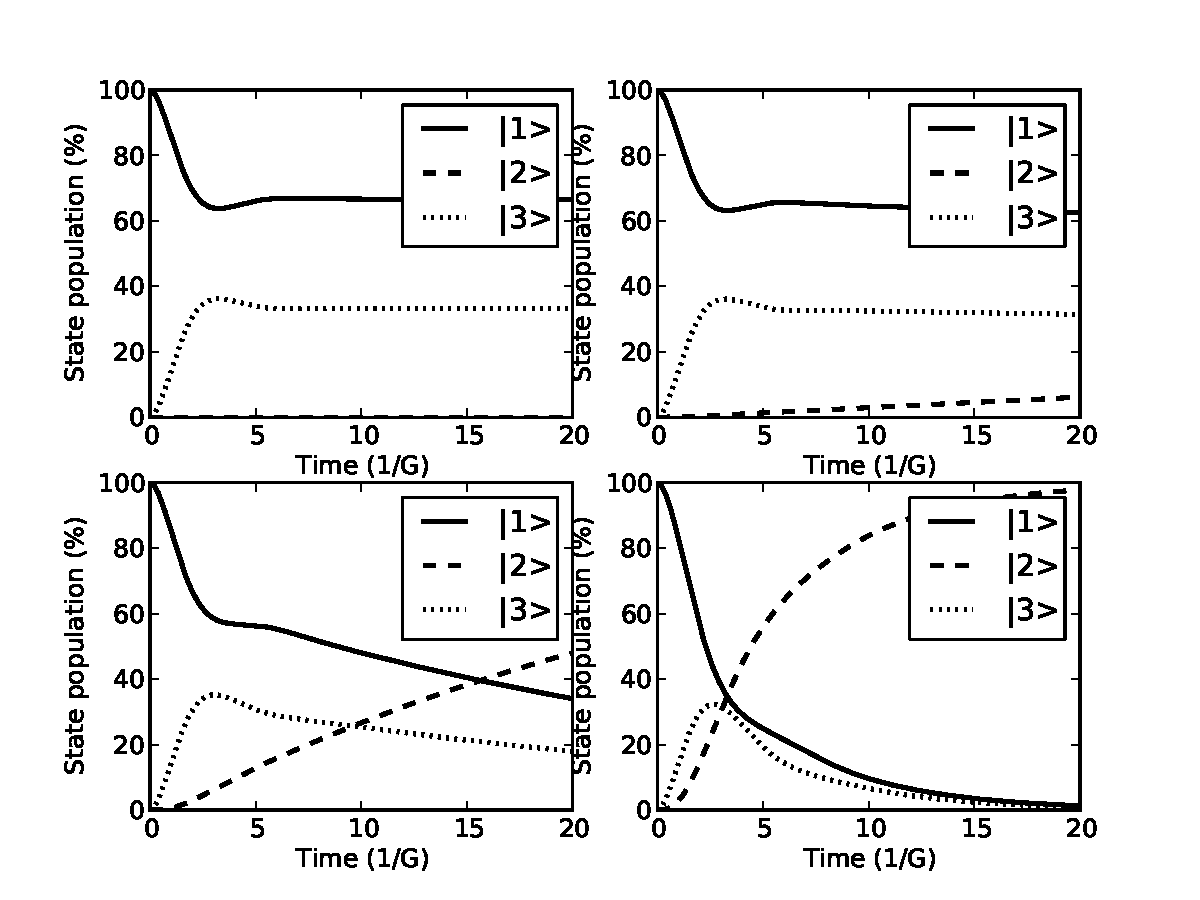
\includegraphics[width=0.65\textwidth]{figures/matt43.pdf}
\caption{Reproducing Figure 4.3 from \cite{McDonnell2003}}
\label{fig:matt43}
\end{center}
\end{figure}

\begin{figure}
\begin{center}
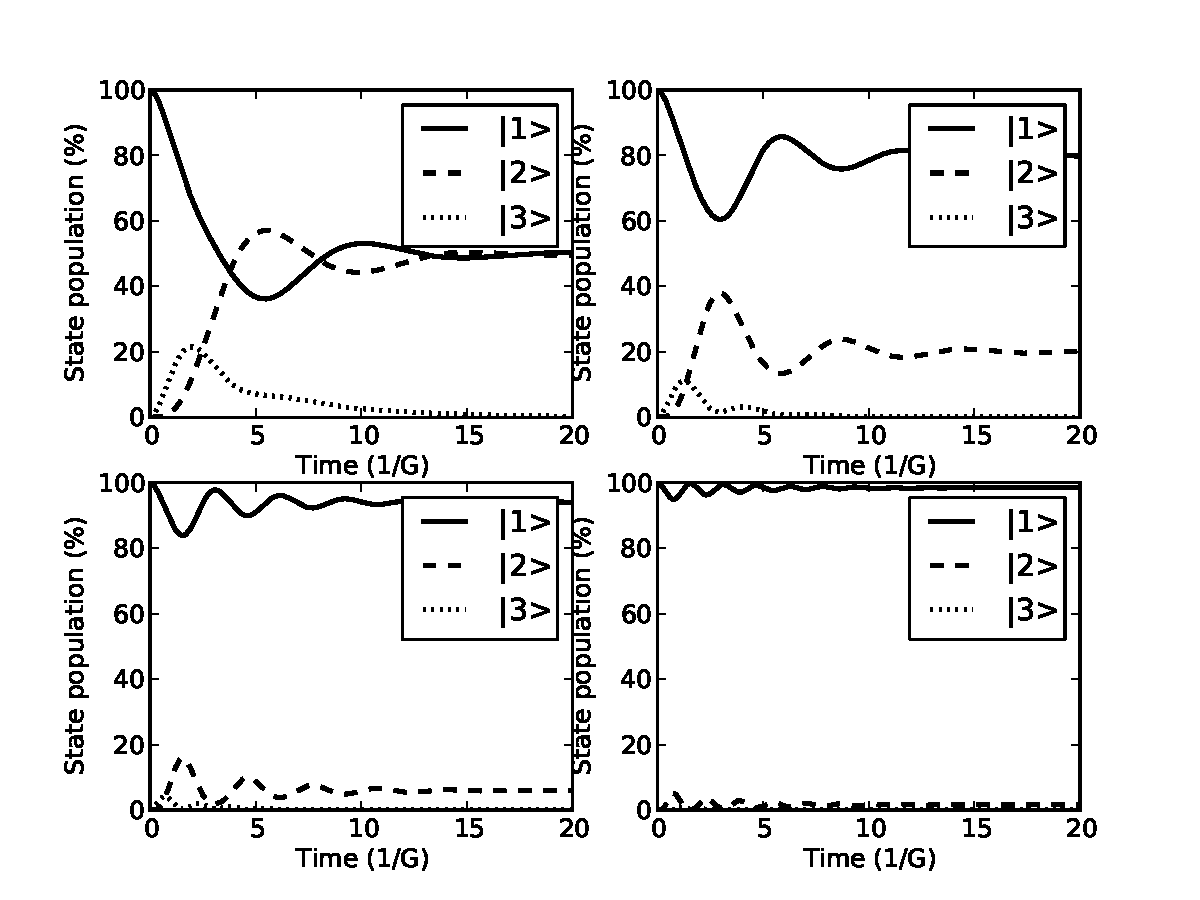
\includegraphics[width=0.65\textwidth]{figures/matt45.pdf}
\caption{Reproducing Figure 4.5 from \cite{McDonnell2003}}
\label{fig:matt45}
\end{center}
\end{figure}

\begin{figure}
\begin{center}
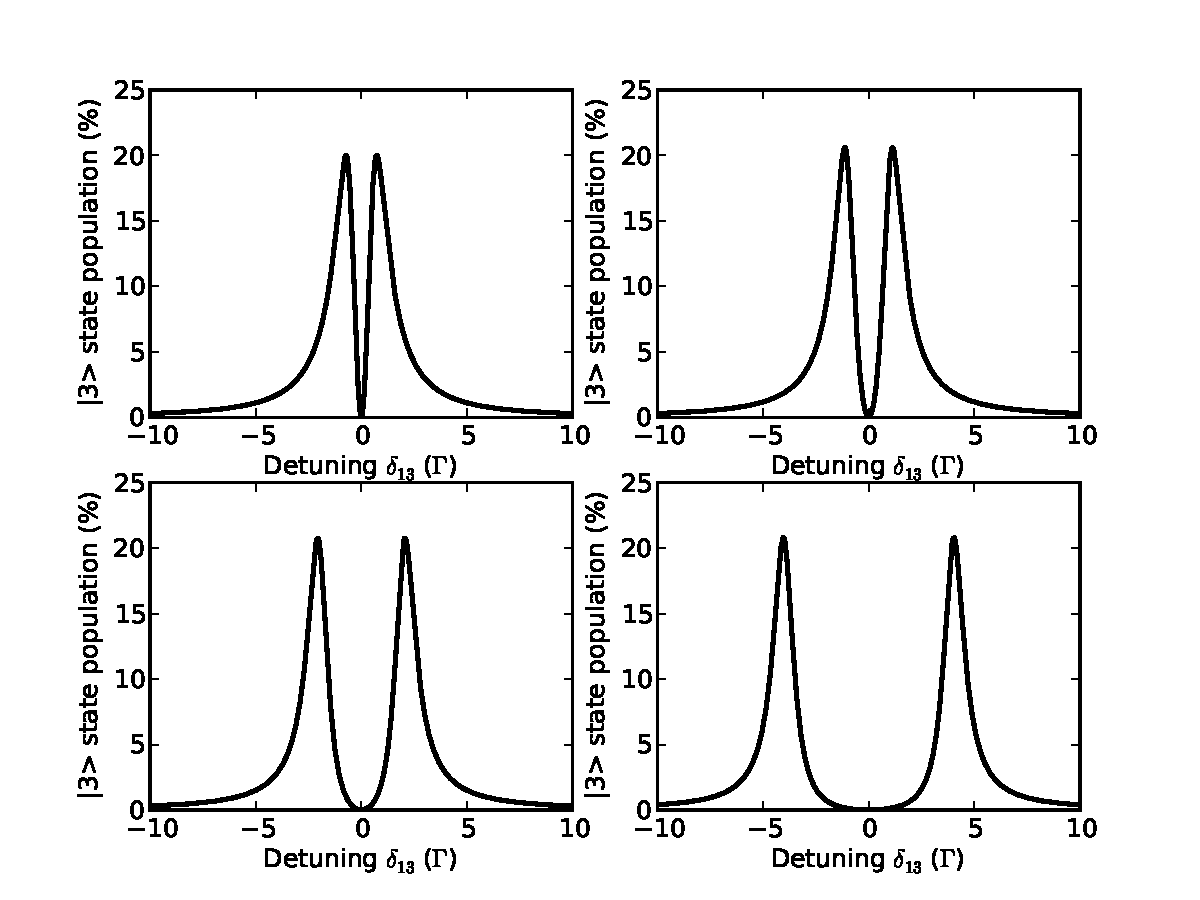
\includegraphics[width=0.65\textwidth]{figures/matt46.pdf}
\caption{Reproducing Figure 4.6 from \cite{McDonnell2003}}
\label{fig:matt46}
\end{center}
\end{figure}

\begin{figure}
\begin{center}
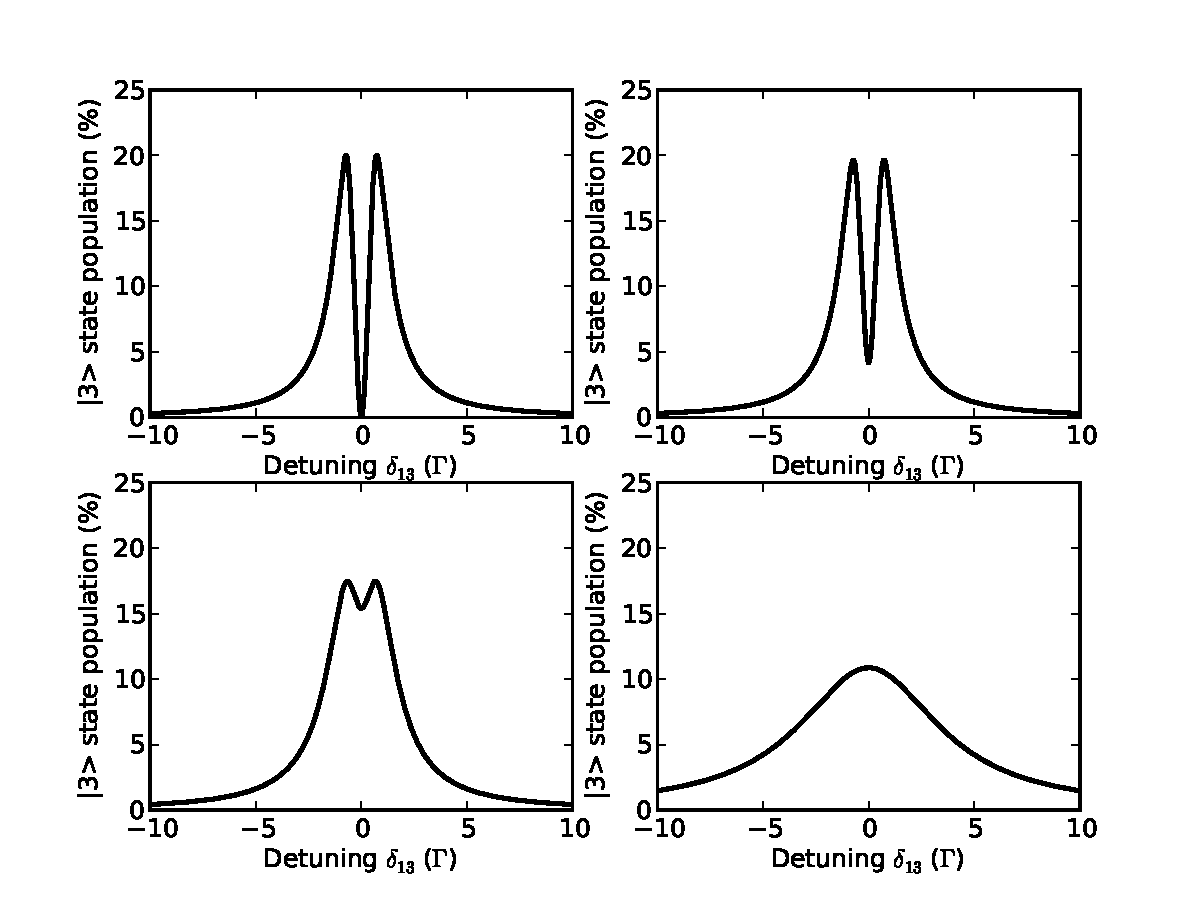
\includegraphics[width=0.65\textwidth]{figures/matt47.pdf}
\caption{Reproducing Figure 4.7 from \cite{McDonnell2003}}
\label{fig:matt47}
\end{center}
\end{figure}

\subsection{CW + pulsed system}
This is \cite{Soares2010}, describing mixed, CW + pulsed laser EIT case.

\subsection{Pulsed rubidium system}
This is \cite{Arissian2006}, describing a mode-locked $^{87}$Rb experiment. Also, there's a newer calculation in \cite{Aumiler2010} that does not add much info just seems to extend on earlier calculations of RB D1 line.


\section{New calculations}

\subsection{No external magnetic field}

In this case the hyperfine magnetic sublevels degenerate, and the quantization axis is set by the light, as opposed to by the magnetic field. The calculation has to be done only between different $F$ levels, which reduces the number of levels, but slighly complicates the interpretation of the input light polarization (at least until I figure it out)

In \cite{Vujicic2007} the authors calculate such a system, and it might be interesting for us since they do compare their theoretical results to experiments, which fit very nicely. The situation is slightlu different, though: strong pumping pulsed laser with fixed repetition rate, tuned weak CW probe laser. The transition strengths between the different $F$ levels are listed in the paper (figure 1), but the normalization is not completely clear to me. The upward coupling streng ratios are properly reproduced by calculating the relative strengths of the transitions as Equation 41 in \cite{Steck2009}:
\begin{equation}
S_{FF'} = (2 F' + 1)(2 J + 1)\left\{ \begin{matrix}  J & J' & 1 \\  F' & F & I \end{matrix}\right\}^2
\end{equation}
where the unprimed and primed symbols represent the starting (lower) and final (upper) states' quantum numbers, respectively. (This gives the $d^2$ thus to get the $\Omega$ Rabi frequency, we got to take the square-root of it? Big question mark.)

The branching ratios for the upper state decay are calculate the same way, reversing the roles of the unprimed and primed symbols.

Useful rules to note: the sum of the coupling to all upper levels is 1, the sum of coupling of an upper level to all lower level is 0. And in case of the D2 line, the $F'=5$ state can only decay to $F=4$.


\subsubsection{4-level Cs system (D1 line)}

From the coupling strengths one can see that this system has strong cross-copling: F=3$\rightarrow$F'=4, and F=4$\rightarrow$F'=3. This would mix the ground state levels much more.


\subsubsection{6-level Cs system (D2 line)}

Strong cross-couplign disappears, probably reducing the ground state level mixing. In the zero temperature regime the carrier frequency seems to be  very important for the observation of dark states. For example, if the carrier is tuned to F=3$\rightarrow$F'=2 or F=4$\rightarrow$F'=5, the dominant transition is that one, and any sideband coupling the other F' states has very tiny effect. Thus even if the ground states are coherently trapped, the upper state has very tiny drop in fluorescence - if any, since the fluorescence is dominated by the F'=2 or F'=5 states that are not affected.



\subsection{Alternative inspirations}

Looking at the literature, there can be systems analogous to ours, who could have solved many of my current questions regarding the inclusion of buffer gas, collisional and pulsed effects.

\subsubsection{Atomic iodine laser}

Coming to my attention a paper \cite{Riley1979} describes theoretical description of atomic iodine laser. That experimental system (as far as I understand at the moment) consists of a cell containing iodine in some molecular form, buffer gas and pulsed pumping. Their question is how this system amplifies the incoming pulse. Switch the iodine molecule to cesium, and amplification to excited state population and one arrives to our experimental setting. I cannot yet be completely sure if they can describe our case as they work in a number of limits. For our case, we need short, saturating pulses. Also, their short pulse is on the time scale of 200 ps, which is two orders of magnitude longer than our ``long'' pulse. Their analysis is done with Maxwell-Bloch equations. It is no surprise, they are interested in the evolution of the electric field. This could do well for us as well, though, especially if our system is really in the optically thick regime (though for that one has to check out \cite{Godone2002} and others). I suppose it would....

For iodine, the relevant lower and upper levels are $^2P_{3/2}$ and $^2P_{1/2}$ respectively (yes, $3/2$ is the lower one). They describe the way they insert collisional dephasing:
\begin{equation}
\dot \rho_{II} = - \gamma_{L} \left(\rho_{II} - \frac{g_{I}}{g_{L}} \rho_{L}\right) 
\end{equation}
where $g_{L} = \sum_{I=3}^{6}g_{I}$, $\rho_{L}=\sum_{I=3}^{6} \rho_{II}$, and $\gamma_{I} = \gamma_{L}$. This applies only to the $P_{3/2}$ state of the iodine, the upper case does not have collisional decay, according to a theoretical analysis of \cite{Yukov1973}. I wonder if similar analysis is possible about the cesium - or has it been done already.

The theoretical results of \cite{Riley1979} show good agreement with their experiment. There is also a paper with apparently further work \cite{Uchiyama1982} that needs further attention.

 

\subsection{Effects to consider}

\subsubsection{Finite beam size}

This could be included as a loss and gain rate with the following properties: loss applies to all states equaly, while gain applies to the ground state levels equally. Here, I think, equality should take into account the degeneracy of the sub-levels if only F states are taken into account.

Probably the correct solution will be more complex than this, as in some paper (reference: forgot, have to find) they include it as a fenomenological diffusion rate.

\subsubsection{Doppler-effects}

This might require integrating (summing) over different velocity classes, though the exact form is modified by the buffer gas collisions.

\subsubsection{Buffer-gas collisions}

This is the trickiest one yet. Buffer gas collisions are properly described in the CW regime, where their two-fold effect is included by hand: pressure-shift and pressure-broadening is thought as a stationary, homogenious effect thus just merged into the other Hamiltonians as shift and larger linewidth. How to handle this when when the laser is pulsed is not completely clear. Previous analysis in \cite{Riley1979} that has most things common with our system don't seem to care about the shift, though need to check more in detail.

\subsubsection{Re-absorption}

Could come up in optically thick medium, though probably much more important if our systems is MOT-trapped Cs instead of conventional gass cell. In the current case it is much lower level effect that can be neglected for the time being.


%% Now... \cite{Berman1986}
%% \begin{lstlisting}[label=test,caption={[short] caption text }]
%% from numpy import *
%% import pylab as pl

%% data = loadtxt('filename.txt')
%% time = data[:, 0]
%% fluo = data[:, 1]
%% pl.plot(time, fluo, 'k-')
%% pl.xlabel('Time (s)')
%% pl.ylabel('Fluorescence (A.U.)')
%% pl.show()
%% \end{lstlisting}

\subsection{Things to check in the futre}
\begin{itemize}
\item Full cesium system
\item Magnetic field
\item Buffer gas effects, shift, broadening/narrowing
\item Higher energy levels for multi-photon processes
\end{itemize}

\newpage
\addcontentsline{toc}{section}{Bibliography}
\bibliographystyle{apalike}
\bibliography{physics_all}

\end{spacing}
\end{document}

%%%%%%%%%%%%%%%%%%%%%%%%%%%%%%%%%%%%%%%%%%%%%%%%%%%%%%%%%%%%%
